\section{Results}\label{sec:results}
All numbers below come from the runs stored in \code{results/} and were produced by
\code{analysis/analyze.py}. Nothing was edited by hand.

\subsection{E1 -- Deployment and UE-to-data-network connectivity}\label{sec:e1}
All twelve 5GC processes and the gNB started; the NG Setup succeeded
(\code{gNB-N2 accepted[10.10.0.2]}, \code{Number of gNBs is now 1}), and the SMF formed PFCP
associations with both UPFs. Listing~\ref{lst:uetable} is the state reported by
\code{nr-cli} after attach. Every UE is \code{RM-REGISTERED}. The multi-slice UE holds
\emph{two} PDU sessions in two pools (10.45.0.4 on eMBB, 10.46.0.3 on URLLC). The negative
test UE \code{badslice} registers but obtains no address.

\begin{lstlisting}[caption={UE and PDU-session state after E1 attach (\code{results/e1/ue\_table.txt}).},label={lst:uetable}]
UE        SUPI                  RM-STATE       PSI  DNN       SST  SD      ADDRESS      IFACE
badslice  imsi-001010000000007  RM-REGISTERED  1    urllc     2    000002  null         -
embb1     imsi-001010000000001  RM-REGISTERED  1    internet  1    000001  10.45.0.2    uesimtun0
embb2     imsi-001010000000002  RM-REGISTERED  1    internet  1    000001  10.45.0.3    uesimtun1
miot1     imsi-001010000000004  RM-REGISTERED  1    iot       3    000003  10.47.0.2    uesimtun3
miot2     imsi-001010000000005  RM-REGISTERED  1    iot       3    000003  10.47.0.3    uesimtun4
multi     imsi-001010000000006  RM-REGISTERED  1    internet  1    000001  10.45.0.4    uesimtun5
multi     imsi-001010000000006  RM-REGISTERED  2    urllc     2    000002  10.46.0.3    uesimtun6
urllc1    imsi-001010000000003  RM-REGISTERED  1    urllc     2    000002  10.46.0.2    uesimtun2
\end{lstlisting}

\noindent The AMF rejects the unsubscribed slice explicitly, and the UE reports the
corresponding 5GMM cause:
\begin{lstlisting}
[amf] [gmm] WARNING: [imsi-001010000000007] Ue requested DNN "urllc" Not Supported OR Not Subscribed in the Slice
[ue ] [nas] [error] MM status received with cause [DNN_NOT_SUPPORTED_OR_NOT_SUBSCRIBED]
\end{lstlisting}

\paragraph{Data flow.} Every PDU session reached the DN: 10/10 ICMP echoes from each of the
seven sessions, with RTT averages of 0.72--0.93\,ms. The same capture proves that the traffic
used the intended user plane (Listing~\ref{lst:gtpu}). eMBB and mIoT packets are tunnelled
to UPF-A (10.10.0.1), and \emph{both} URLLC sessions (urllc1 and multi's second session) to
UPF-B (10.10.0.3). Each session has its own TEID pair. iperf3 downlink goodput was
138\,Mbit/s on eMBB, 18.7\,Mbit/s on URLLC and 2.10\,Mbit/s on mIoT. These match the binding
cap of each slice: the tc MBR of 150 and 20\,Mbit/s, and the 2\,Mbit/s Session-AMBR for mIoT.
HTTP requests from each slice through N6 and NAT to a public web server returned
\code{200} in 72--80\,ms.

\begin{lstlisting}[caption={GTP-U-encapsulated pings per N3 endpoint, outer$\rightarrow$inner
addresses (\code{results/e1/gtpu\_per\_upf.txt}; uplink rows shown).},label={lst:gtpu}]
 10 10.10.0.2->10.10.0.1  inner 10.45.0.2->192.168.100.2  teid 0x00006eee   eMBB  -> UPF-A
 10 10.10.0.2->10.10.0.1  inner 10.45.0.4->192.168.100.2  teid 0x0000a57f   eMBB  -> UPF-A (multi)
  9 10.10.0.2->10.10.0.3  inner 10.46.0.2->192.168.100.2  teid 0x00000600   URLLC -> UPF-B
 10 10.10.0.2->10.10.0.3  inner 10.46.0.3->192.168.100.2  teid 0x0000f718   URLLC -> UPF-B (multi)
 10 10.10.0.2->10.10.0.1  inner 10.47.0.2->192.168.100.2  teid 0x000044f9   mIoT  -> UPF-A
\end{lstlisting}

\subsection{E2 -- Signalling: registration, session establishment and slice selection}\label{sec:e2}
Figure~\ref{fig:ladder} is the message sequence of the multi-slice UE, reconstructed directly
from the capture. It shows the complete 5G registration (TS~23.502~\S4.2.2.2~\cite{ts23502}).
InitialUEMessage carries the Registration Request with the SUCI and the requested NSSAI. The
AMF fetches 5G-AKA vectors via AUSF/UDM (Authentication Request/Response). The Security Mode
Command then selects NIA2/NEA0. InitialContextSetupRequest carries the Registration Accept,
whose \textbf{Allowed NSSAI} contains exactly the subscribed S-NSSAIs: \code{SST 1/SD 000001} and
\code{SST 2/SD 000002} for this UE.
Table~\ref{tab:nssai} lists the NSSAI each UE received. The UE subscribed only to eMBB that
asked for URLLC gets \code{SST 1} as Allowed NSSAI and \code{SST 2/SD 000002} as
\textbf{Rejected NSSAI} (cause 0, ``S-NSSAI not available in the current PLMN''). That is
exactly the behaviour TS~24.501 specifies for a non-subscribed S-NSSAI~\cite{ts24501}.

\begin{table}[H]\centering\small
\caption{NSSAI in each Registration Accept, decoded from the capture (\code{results/e1/allowed\_nssai.txt}).}\label{tab:nssai}
\begin{tabular}{lll}
\toprule
UE (RAN-UE-NGAP-ID) & Allowed NSSAI (SST/SD) & Rejected NSSAI\\
\midrule
embb1 (1), embb2 (2) & 1/000001 & --\\
urllc1 (3) & 2/000002 & --\\
miot1 (4), miot2 (5) & 3/000003 & --\\
multi (6) & 1/000001, 2/000002 & --\\
badslice (7) & 1/000001 & 2/000002 (cause 0)\\
\bottomrule
\end{tabular}
\end{table}

\noindent Two PDU Session Establishment Requests follow (one per S-NSSAI/DNN). The SMF then opens one
PFCP session on \textbf{UPF-B} (127.0.0.17, URLLC) and one on \textbf{UPF-A} (127.0.0.7,
eMBB), and each N2 PDUSessionResourceSetupRequest gives the gNB the corresponding UPF N3
address.

\begin{figure}[H]\centering
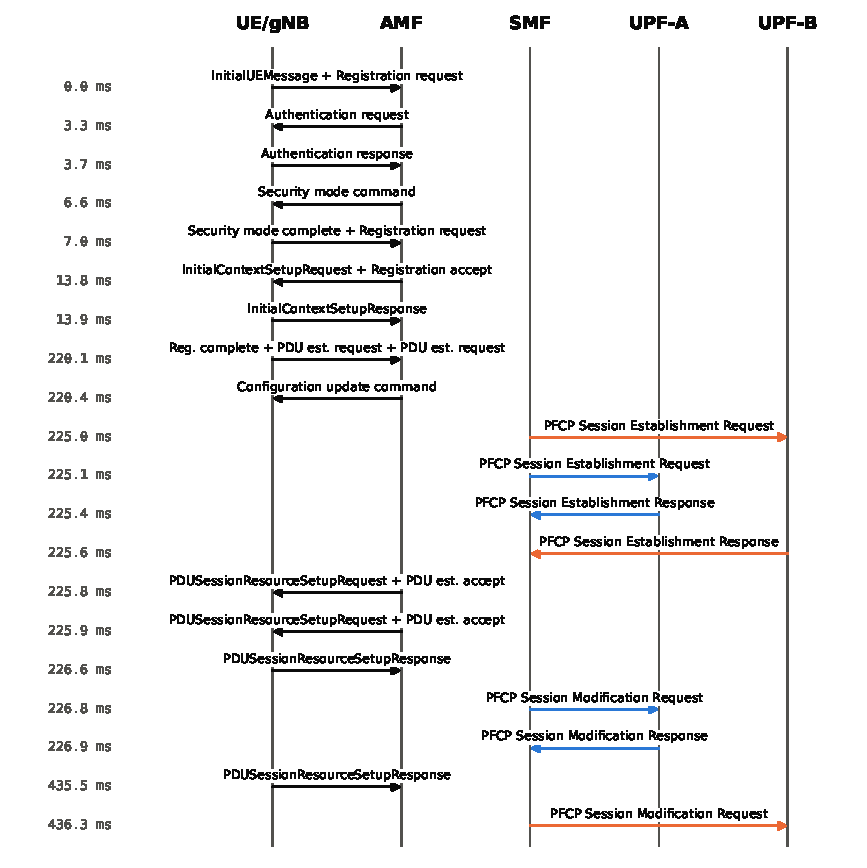
\includegraphics[width=0.76\linewidth]{figures/fig_ladder_multi.pdf}
\caption{N2 (NGAP/NAS) and N4 (PFCP) messages for UE \code{imsi-001010000000006}, extracted from
\code{results/e1/attach.pcapng}. Orange arrows: PFCP to the dedicated URLLC UPF-B; blue: shared
UPF-A. Times are relative to the InitialUEMessage.}\label{fig:ladder}
\end{figure}

Over all UEs the capture contains 5 PFCP Session Establishments towards UPF-A and 2 towards
UPF-B, which is exactly the number of eMBB+mIoT and URLLC sessions. Table~\ref{tab:sigtime}
gives the procedure latencies. Registration completes in 7--17\,ms and a PDU session in
6--15\,ms. The $\approx$200\,ms gap between Registration Accept and the first PDU request is
UERANSIM's own timer, not network latency. Table~\ref{tab:sbi} lists the service-based
operations behind these procedures (N8/N10/N12/N13 UDM/UDR/AUSF, N11 AMF$\rightarrow$SMF,
N7/N15 PCF, BSF binding). Every SBI request is counted twice, because the capture sees both
hops (NF$\rightarrow$SCP$\rightarrow$NF).

\begin{table}[H]\centering\small
\begin{minipage}[t]{0.52\linewidth}\centering
\caption{Procedure latency per UE (from N2 timestamps).}\label{tab:sigtime}
\resizebox{\linewidth}{!}{\begin{tabular}{llrcl}
\toprule
UE & SUPI & Registration [ms] & PDU sessions & PDU setup [ms] \\
\midrule
embb1 & imsi-001010000000001 & 15.3 & 1 & 15.2 \\
embb2 & imsi-001010000000002 & 12.1 & 1 & 9.2 \\
urllc1 & imsi-001010000000003 & 15.5 & 1 & 7.9 \\
miot1 & imsi-001010000000004 & 12.8 & 1 & 10.8 \\
miot2 & imsi-001010000000005 & 7.3 & 1 & 10.4 \\
multi & imsi-001010000000006 & 13.8 & 2 & 6.4, 215.4 \\
badslice & imsi-001010000000007 & 17.0 & 0 & rejected \\
\bottomrule
\end{tabular}
}
\end{minipage}\hfill
\begin{minipage}[t]{0.45\linewidth}\centering
\caption{Most frequent SBI operations (excluding NRF heartbeats).}\label{tab:sbi}
\resizebox{\linewidth}{!}{\begin{tabular}{llr}
\toprule
SBI API & Operation & Count \\
\midrule
nudr-dr & GET /subscription-data/\{supi\} & 56 \\
nudr-dr & GET /policy-data/ues & 28 \\
nudm-sdm & POST /\{supi\}/sdm-subscriptions & 28 \\
nudr-dr & PUT /subscription-data/\{supi\} & 27 \\
nudm-uecm & PUT /\{supi\}/registrations & 22 \\
nsmf-pdusession & POST /sm-contexts & 14 \\
nsmf-pdusession & POST /sm-contexts/\{id\} & 14 \\
namf-comm & POST /ue-contexts/\{supi\} & 14 \\
nbsf-management & POST /pcfBindings & 14 \\
npcf-smpolicycontrol & POST /sm-policies & 14 \\
nudm-sdm & GET /\{supi\}/sm-data & 14 \\
nausf-auth & POST /ue-authentications & 14 \\
\bottomrule
\end{tabular}
}
\end{minipage}
\end{table}

\subsection{E6 -- Temporal traffic profiles per slice}
Figure~\ref{fig:e6} confirms that each generator reproduces its service class (scenario S1,
90\,s). eMBB alternates 20\,s downloads at the 150\,Mbit/s slice cap (two UEs share it) with
5\,s idle gaps. URLLC is a perfectly periodic 100 echoes/s at 0.05\,Mbit/s. mIoT shows the
Poisson-modulated arrival of 400 sensors (mean 38 reports/s for 200 devices $\times$ 2 gateways
at a 10\,s mean period; theory 40/s).

\begin{figure}[H]\centering
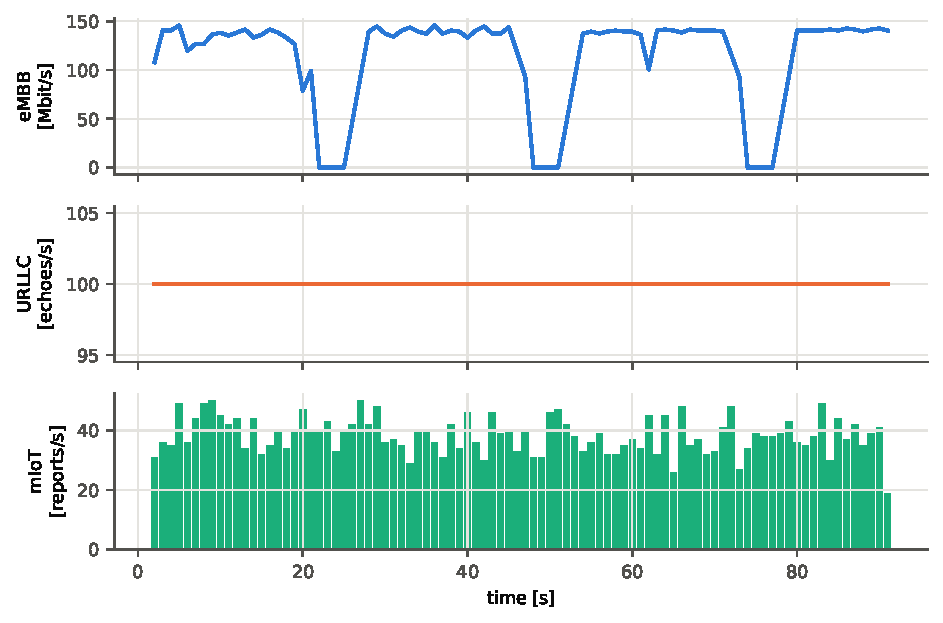
\includegraphics[width=0.74\linewidth]{figures/fig_e6_profiles.pdf}
\caption{Per-slice offered traffic in scenario S1 (E6).}\label{fig:e6}
\end{figure}

\subsection{E3 -- Isolation of URLLC and mIoT from an eMBB surge}\label{sec:e3}
Figure~\ref{fig:e3} and Table~\ref{tab:e3} show URLLC and mIoT latency before, during and
after an eMBB surge of 2 UEs $\times$ 4 TCP streams. The surge is held at the eMBB slice MBR
($\approx$141\,Mbit/s mean). Neither slice lost a single packet, and their p99 stayed below
1.1\,ms throughout the load phase. The URLLC p99 target of Table~\ref{tab:req} (10\,ms) was
met in every per-second window of the load phase (worst 1.43\,ms). The only violations were
isolated spikes of 13--19\,ms in the \emph{idle} phases. Latency is visibly \emph{lower} under
load (p50 0.32 vs.\ 1.08\,ms). Control experiment E7 explains this (Table~\ref{tab:e7}): pure
CPU busy-loops with no network traffic lower the URLLC p50 from 1.08 to 0.10\,ms. The idle
penalty is therefore CPU idle-state wake-up latency in the VM, not a property of the 5G
stack.

\begin{figure}[H]\centering
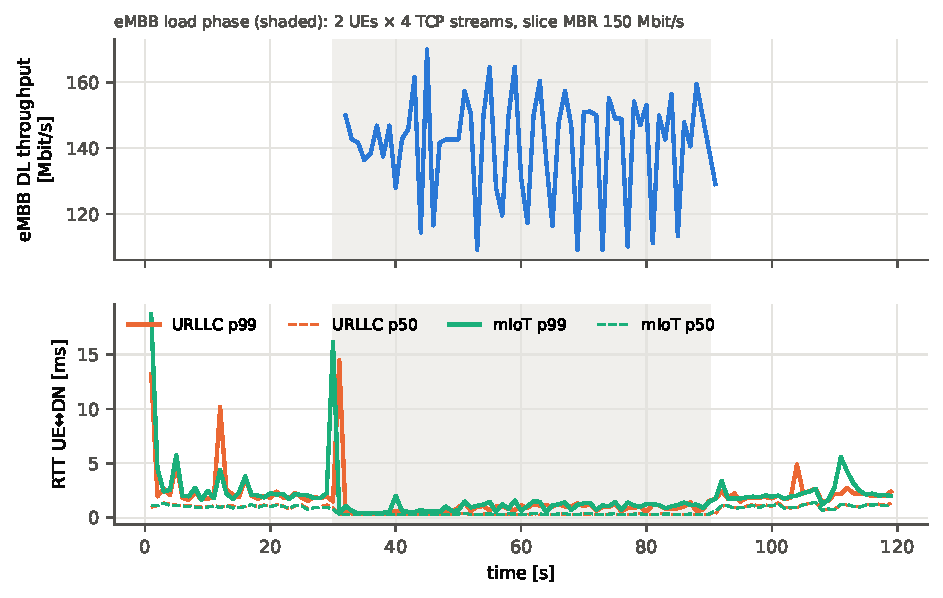
\includegraphics[width=0.78\linewidth]{figures/fig_e3_isolation.pdf}
\caption{E3: eMBB surge (top) and URLLC/mIoT RTT (bottom). Shaded: eMBB load phase.}\label{fig:e3}
\end{figure}

\begin{table}[H]\centering\small
\caption{E3 latency by phase (medians of per-second values).}\label{tab:e3}
\begin{tabular}{llrrrr}
\toprule
Slice & Phase & RTT p50 [ms] & RTT p99 [ms] & worst p99 [ms] & Loss [\%] \\
\midrule
URLLC & idle (0–30 s) & 1.08 & 1.95 & 13.22 & 0.00 \\
URLLC & eMBB load (30–90 s) & 0.32 & 0.86 & 1.43 & 0.00 \\
URLLC & after (90–120 s) & 1.11 & 2.06 & 4.90 & 0.00 \\
mIoT & idle (0–30 s) & 1.05 & 2.19 & 18.70 & 0.00 \\
mIoT & eMBB load (30–90 s) & 0.33 & 1.05 & 2.02 & 0.00 \\
mIoT & after (90–120 s) & 1.09 & 2.04 & 5.58 & 0.00 \\
\bottomrule
\end{tabular}

\end{table}
\begin{table}[H]\centering\small
\caption{E7 control experiment: URLLC RTT vs.\ CPU state, without any other traffic.}\label{tab:e7}
\begin{tabular}{lrr}
\toprule
Condition & RTT p50 [ms] & RTT p99 [ms] \\
\midrule
idle (0–30 s) & 1.078 & 2.06 \\
CPU busy-loops, no traffic (30–60 s) & 0.095 & 2.16 \\
idle again (60–90 s) & 1.412 & 1.94 \\
\bottomrule
\end{tabular}

\end{table}

\subsection{E4 -- Live slice-parameter changes}\label{sec:e4}
With all three slices active, two parameters were changed live through the same API the
sandbox uses (Fig.~\ref{fig:e4}). At $t$\,=\,40\,s the eMBB MBR was cut from 150 to
30\,Mbit/s. eMBB goodput fell from 137.6 to 28.1\,Mbit/s (94\,\% of the new cap) within one
1-s sample, with no session re-establishment. URLLC kept exactly 100 echoes/s and mIoT
$\approx$40 reports/s in every phase.
At $t$\,=\,80\,s the URLLC slice received +5\,ms one-way delay in each direction. URLLC p50
rose from 1.2 to 11.7\,ms ($\approx$\,+10\,ms, as configured), while the mIoT p50 stayed at
1.3\,ms. Each change therefore affected only the targeted slice. The small rise of URLLC/mIoT
latency after $t$\,=\,40\,s is again the CPU artefact: less eMBB traffic leaves the VM more
idle.

\begin{figure}[H]\centering
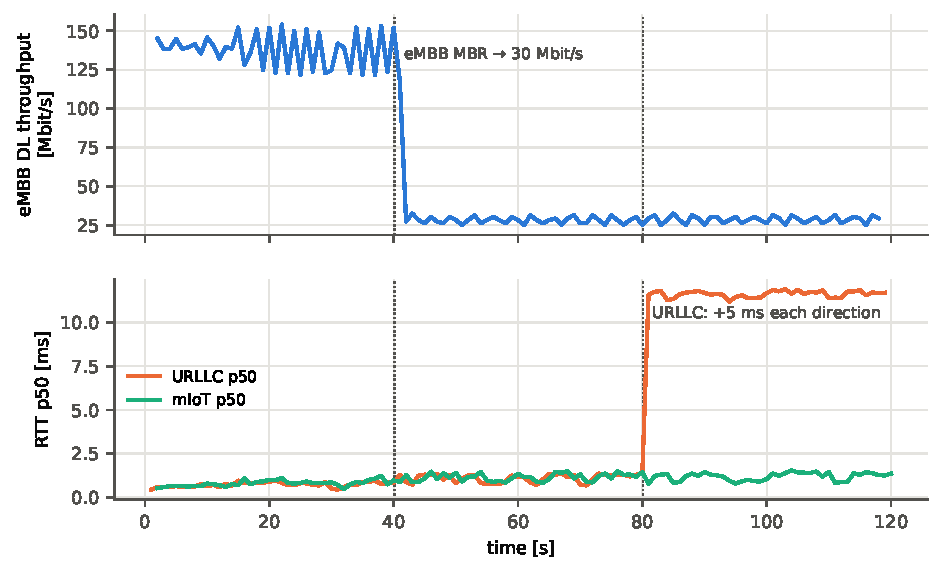
\includegraphics[width=0.78\linewidth]{figures/fig_e4_live.pdf}
\caption{E4: live MBR change on eMBB at $t$\,=\,40\,s and live delay change on URLLC at
$t$\,=\,80\,s (dotted lines, from the event log).}\label{fig:e4}
\end{figure}

\subsection{E5 -- Dedicated vs.\ shared user plane for URLLC}\label{sec:e5}
To test the design decision of \S\ref{sec:slices}, the URLLC probe (200\,Hz) ran under an
identical eMBB overload in two configurations. In \emph{dedicated} mode URLLC is anchored on
UPF-B. In \emph{shared} mode the SMF/UPF-A configs put the \code{urllc} DNN on UPF-A, the
same UPF as eMBB. To make the offered load identical in both modes, eMBB was a fixed-rate UDP
flood (2 UEs $\times$ 500\,Mbit/s downlink) with Session-AMBR and the tc MBR lifted. The
modes were alternated over three repetitions each, so that host drift affects both equally.
During the load phase the VM had no idle CPU. The iperf3 senders alone used about 3 of the 4
vCPUs, followed by \code{open5gs-upfd} (23--42\,\%) and \code{nr-gnb} (20--41\,\%). This is a
deliberately extreme stress test, not an operating point.

\begin{figure}[H]\centering
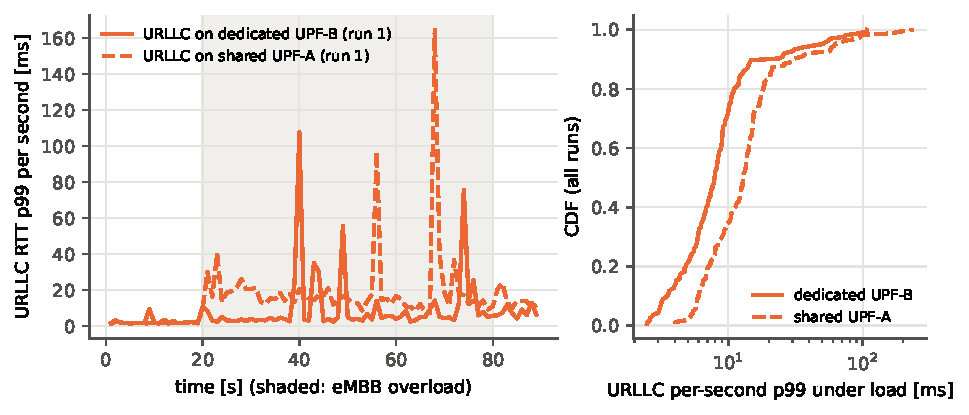
\includegraphics[width=0.86\linewidth]{figures/fig_e5_upf.pdf}
\caption{E5: URLLC per-second p99 RTT in the first run of each mode (left), and the CDF over
all three runs per mode (right, log scale). Shaded: eMBB overload.}\label{fig:e5}
\end{figure}

\begin{table}[H]\centering\small
\caption{E5 summary (mean $\pm$ s.d.\ over 3 runs per mode of the per-run median during load).}\label{tab:e5}
\resizebox{\linewidth}{!}{\begin{tabular}{lrrrrrrr}
\toprule
URLLC user plane & runs & load p50 [ms] & load p99 [ms] & p95 of p99 [ms] & worst p99 [ms] & loss [\%] & eMBB [Mbit/s] \\
\midrule
dedicated & 3 & 1.50 ± 0.86 & 7.42 ± 2.34 & 43.21 ± 9.97 & 107.5 & 11.937 & 58 \\
shared & 3 & 3.77 ± 1.90 & 11.78 ± 4.27 & 59.50 ± 22.36 & 237.4 & 4.831 & 41 \\
\bottomrule
\end{tabular}
}
\end{table}

Sharing the UPF made URLLC latency worse (Fig.~\ref{fig:e5}, Table~\ref{tab:e5}). Pooled over
all load seconds, the median of the per-second p99 rose from 7.9\,ms (dedicated) to 12.9\,ms
(shared). The share of seconds meeting the 10\,ms p99 target fell from 72\,\% to 35\,\%
(Mann--Whitney $p<10^{-11}$; the per-second samples are autocorrelated, so this overstates
the significance). At the correct statistical unit (one value per run, $n$\,=\,3 per mode),
the shared configuration has a 2.5$\times$ higher median RTT and a 1.6$\times$ higher p99, but
Welch's test gives $p$\,=\,0.16 and 0.22. The direction is consistent in two of three
pairs, but more repetitions would be needed to claim significance. URLLC \emph{loss} was
substantial in both modes and, unexpectedly, higher with the dedicated UPF (11.9 vs.\
4.8\,\%). Packets are dropped in components that both modes share, the user-space gNB/UE
(RLS) and the starved CPU, which UPF separation cannot isolate.

